\documentclass{article}
\usepackage{amsmath}
\usepackage{graphicx}
\usepackage{siunitx}
\graphicspath{{./images/}}

\title{University Physics with Modern Physics Electromagnetism Notes}
\author{Chris Doble}
\date{December 2022}

% The Coulomb constant
\newcommand{\ke}{\frac{1}{4 \pi \epsilon_0}}

\begin{document}

\maketitle

\tableofcontents

\setcounter{section}{20}
\section{Electric Charge and Electric Field}

\subsection{Electric Charge}

\begin{itemize}
  \item Electrons have a much smaller mass than neutrons and protons

  \item Neutrons and protons have a very similar mass

  \item Electrons and protons have the same magnitude of charge

  \item The number of protons in an atom determins its \textbf{atomic number}

  \item If an electron is added to a neutral atom it becomes a \textbf{negative ion}, if one is removed it becomes a \textbf{positive ion} — this is called \textbf{ionisation}

  \item The \textbf{principle of conservation of charge} states that the algebraic sum of all the electric charges in any closed system is constant

  \item The electron or proton's magnitude of charge is a natural unit of charge — every observable amount of electric charge is an integer multiple of this
\end{itemize}

\subsection{Conductors, Insulators, and Incuded Charges}

\begin{itemize}
  \item \textbf{Conductors} pemit easy movement of charge, \textbf{insulators} do not

  \item Holding a charged object near an uncharged object causes free electrons in the latter to move away/towards the former, resulting in a net charge on either side — this is called \textbf{induced charge}
\end{itemize}

\subsection{Coulomb's Law}

\begin{itemize}
  \item The SI unit of charge is called one \textbf{coulomb} (1 C) and is defined such that $1.602176634\times10^{-19}$ C is equal to the charge of an electron or proton

  \item \textbf{Coulomb's law} describes the electric force between two point charges \[F = \frac{1}{4\pi\epsilon_0}\frac{|q_1q_2|}{r^2}\] where the \textbf{electric constant} $\epsilon_0 = 8.854 \times 10^{-12}\,\textrm{C}^2/\textrm{N}\cdot \textrm{m}^2$, $q_1$ and $q_2$ are the magnitudes of the charges, and $r$ is the distance between them

  \item The electric force is always directed along the line between the two charges, attracting opposite charges and repelling like charges

  \item $\frac{1}{4\pi\epsilon_0}$ can be approximated as $9.0 \times 10^9\,\textrm{N}\cdot\textrm{m}^2/\textrm{C}^2$

  \item The principle of superposition of forces also applies to electric charges
\end{itemize}

\subsection{Electric Field and Electric Forces}

\begin{itemize}
  \item The electric force on a charged object is exerted by the electric field created by other charged objects

  \item We can determine if there is an electric field at a point by placing a test charge $q_0$ there and seeing if it experiences an electric force — the electric field at that point (the electric force per unit charge) is then given by \[\mathbf{E} = \frac{\mathbf{F}}{q_0}\]

  \item Rearranging, the force experienced by a charge $q_0$ at a point is given by \[\mathbf{F} = q_0\mathbf{E}\]

  \item When considering an electric field produced by a point charge, the location of the point charge is called the \textbf{source point} and the location at which we're trying to determine the field is called the \textbf{field point}

  \item The electric field produced by a point charge is given by \[\mathbf{E} = \frac{1}{4\pi\epsilon_0} \frac{q}{r^2}\hat{\mathbf{r}}\] where $q$ is the charge of the point charge, $r$ is the distance between the source and field points, and $\hat{\mathbf{r}}$ is the unit vector from the source to the field point

  \item Unlike Coulomb's law this equation doesn't use the absolute value of $q$ meaning that the electric fields of positive charges point away from the charge, while those of negative charges point towards them

  \item In electrostatics, the electric field inside the material of a conductor (but not holes within the material) is $\mathbf{0}$
\end{itemize}

\subsection{Electric-Field Calculations}

\begin{itemize}
  \item The \textbf{principle of superposition of electric fields} states that the total electric field at a point $P$ is the vector sum of the fields at $P$ due to each point charge in the charge distribution \[\mathbf{E} = \mathbf{E}_1 + \mathbf{E}_2 + \cdots\]

  \item For a line charge distribution the \textbf{linear charge density} is represented by $\lambda$ (the charge per unit length, measured in $\textrm{C}/\textrm{m}$)

  \item For a surface charge distribution the \textbf{surface charge density} is represented by $\sigma$ (the charge per unit area, measured in $\textrm{C}/\textrm{m}^2$)

  \item For a volume charge distribution the \textbf{volume charge density} is represented by $\rho$ (the charge per unit volume, measured in $\textrm{C}/\textrm{m}^3$)

  \item The electric field of an infinitely long line charge along the $y$-axis is \[E = \frac{\lambda}{2\pi\epsilon_0 r}\]
\end{itemize}

\subsection{Electric Field Lines}

\begin{itemize}
  \item An \textbf{electric field line} is a line drawn through space such that its tangent at any point is in the direction of the electric field vector at  that point

  \item Fewer lines are drawn in areas where the electric field is weak and more lines are drawn in areas where it's strong
\end{itemize}

\subsection{Electric Dipoles}

\begin{itemize}
  \item An \textbf{electric dipole} is a pair of point charges of equal magnitude $q$ and opposite sign separated by a distance $d$

  \item The net force on an electric dipole in a uniform electric field is $\mathbf{0}$

  \item The \textbf{electric dipole moment} $\mathbf{p}$ of an electric dipole is a vector directed from the negative charge to the positive charge with magnitude $qd$

  \item The net torque on an electric dipole in a uniform electric field is $\mathbf{p} \times \mathbf{E}$ or $qEd\sin\phi$ where $\phi$ is the angle between the electric dipole and the electric field

  \item The potential energy of an electric dipole in a uniform electric field is \[U = -\mathbf{p} \cdot \mathbf{E}\]
\end{itemize}

\section{Gauss's Law}

\subsection{Calculating Electric Flux}

\begin{itemize}
  \item The electric flux of a uniform electric field through a flat surface $A$ is \[\Phi_E = \mathbf{E} \cdot \mathbf{A}\] where $\mathbf{A}$ is normal to $A$ and has a magnitude equal to its area

  \item The electric flux of a nonuniform electric field through a curved surface $A$ is \[\Phi_E = \int \mathbf{E} \cdot \mathbf{dA}\]
\end{itemize}

\subsection{Gauss's Law}

\begin{itemize}
  \item Gauss's law states that the total electric flux through a closed surface is equal to the total electric charge enclosed by the surface divided by $\epsilon_0$ \[\Phi_E = \oint \mathbf{E} \cdot \mathbf{dA} = \frac{Q_\textrm{enc}}{\epsilon_0}\]
\end{itemize}

\subsection{Applications of Gauss's Law}

\begin{itemize}
  \item Gauss's law can be used in two ways:

        \begin{itemize}
          \item If we know the charge distribution and it has enough symmetry to let us evaluate the integral in Gauss's law, we can find the field

          \item If we know the field, we can use Gauss's law to find the charge distribution
        \end{itemize}

  \item Under electrostatics, excess charge always lies of the surface of a conductor

  \item The electric field of an infinite line charge is \[\mathbf{E} = \ke \frac{2 \lambda}{r} \hat{\mathbf{r}}\]
\end{itemize}

\subsection{Charges on Conductors}

\begin{itemize}
  \item If there is excess charge at rest on a conductor, all of that charge must lie on the surface of the conductor and the electric field inside the conductor must be zero. If there is a cavity inside the conductor, the net charge on the cavity walls equals the amount of charge enclosed by the cavity

  \item Charges outside a conductor have no effect on the interior of the conductor, even if it has a cavity inside — this is why Faraday cages work

  \item At the surface of a conductor, the component of the electric field that is perpendicular to the surface is \[E_\perp = \frac{\sigma}{\epsilon_0}\]
\end{itemize}

\section{Electric Potential}

\subsection{Electric Potential Energy}

\begin{itemize}
  \item The electric potential energy of two point charges is \[U = \ke \frac{q_1 q_2}{r}\]

  \item The electric potential energy of a point charge $q_0$ and a collection of charges $q_1$, $q_2$, etc. is \[U = \frac{q_0}{4 \pi \epsilon_0} \left( \frac{q_1}{r_1} + \frac{q_2}{r_2} + \cdots \right) = \frac{q_0}{4 \pi \epsilon_0} \sum_i \frac{q_i}{r_i}\]

  \item For every electric field due to a static charge distribution, the force exterted by that field is conservative

  \item The total electric potential energy of a collection of charges $q_1$, $q_2$, etc. is \[U = \ke \sum_{i < j} \frac{q_i q_j}{r_{ij}}\] where $r_{ij}$ is the distance between $q_i$ and $q_j$
\end{itemize}

\subsection{Electric Potential}

\begin{itemize}
  \item \textbf{Potential} is potential energy per unit charge

  \item The unit of potential is the \textbf{volt}, equal to 1 joule per coulomb

  \item The potential difference between two points $V_{ab} = V_a - V_b$ is called the potential of $a$ with respect to $b$ and equals the amount of work done by the electric force when a unit ($\qty{1}{C}$) of charge moves from $a$ to $b$

  \item The electric potential due to a point charge is \[V = \ke \frac{q}{r}\]

  \item The electric potential due to a collection of point charges is \[V = \ke \sum_i \frac{q_i}{r_i}\]

  \item The electric potential due to a continuous charge distribution is \[V = \ke \int \frac{dq}{r}\]

  \item The electric potential difference between two points is given by \[V_a - V_b = \int_a^b \mathbf{E} \cdot d\mathbf{l} = \int_a^b E \cos \phi \,dl\]

  \item Positive charges tend to ``fall'' from high- to low-potential regions while negative charges do the opposite

  \item When a particle with charge $e = \qty{1.602e-19}{C}$ moves between two points with a potential difference of $\qty{1}{V} = \qty{1}{J/C}$ the change in energy is $U_a - U_b = qV_{ab} = (\qty{1.602e-19}{C})(\qty{1}{J/C}) = \qty{1.602e-19}{J}$ which is called 1 \textbf{electron volt}
\end{itemize}

\setcounter{subsection}{3}
\subsection{Equipotential Surfaces}

\begin{itemize}
  \item An \textbf{equipotential surface} is a three-dimensional surface on which the electric potential is the same at every point

  \item Because electric potential energy doesn't change as a test charge moves over an equipotential surface, the electric field can do no work and thus \textbf{field lines and equipotential surfaces are always perpendicular}

  \item When all charges are at rest, the surface of a conductor is an equipotential surface

  \item When all charges are at rest, the entire solid volume of a conductor is at the same potential
\end{itemize}

\subsection{Potential Gradient}

\begin{itemize}
  \item The relationship between $\mathbf{E}$ and $V$ is given by \[\mathbf{E} = -\nabla V = -\left( \frac{\partial V}{\partial x} \hat{\mathbf{i}} + \frac{\partial V}{\partial y} \hat{\mathbf{j}} + \frac{\partial V}{\partial z} \hat{\mathbf{k}} \right)\]

  \item If $E$ has a radial component $E_r$ with respect to an axis or a point and $r$ is the distance from that axis or point, then \[E_r = -\frac{\partial V}{\partial r}\]
\end{itemize}

\section{Capacitance and Dielectrics}

\subsection{Capacitors and Capacitance}

\begin{itemize}
  \item Any two conductors separated by an insulator (or a vacuum) form a \textbf{capacitor}

  \item The \textbf{capacitance} of a capacitor measures its ability to store charge \[C = \frac{Q}{V_{AB}}\]

  \item Capacitance is measured in \textbf{farads} where \[\qty{1}{F} = \qty{1}{C/V}\]

  \item The capacitance of a parallel plate capacitor in a vacuum is \[C = \epsilon_0 \frac{A}{d}\]
\end{itemize}

\subsection{Capacitors in Series and Parallel}

\begin{itemize}
  \item In a series connection, the magnitude of charge on all plates is the same

  \item The \textbf{equivalent capacitance} of a combination of capacitors is the capacitance of a single capacitor that would have equivalent behaviour

  \item In a series connection, the reciprocal of the equivalent capacitance equals the sum of the reciprocals of the individual capacitances \[\frac{1}{C_\textrm{eq}} = \frac{1}{C_1} + \frac{1}{C_2} + \cdots\] meaning the equivalent capacitance is always less than any individual capacitance

  \item In a parallel connection, the potential difference is the same for all capacitors

  \item In a parallel connection, the equivalent capacitance equals the sum of the individual capacitances \[C_\textrm{eq} = C_1 + C_2 + \cdots\] meaning the equivalent capacitance is always greater than any individual capacitance
\end{itemize}

\subsection{Energy Storage in Capacitors and Electric-Field Energy}

\begin{itemize}
  \item The potential energy stored in a capacitor is \[U = \frac{Q^2}{2 C} = \frac{1}{2} C V^2 = \frac{1}{2} Q V\]

  \item The \textbf{energy density} of a parallel plate capacitor is its energy per unit volume \[u = \frac{\frac{1}{2} C V^2}{A d} = \frac{1}{2} \epsilon_0 E^2\]
\end{itemize}

\subsection{Dielectrics}

\begin{itemize}
  \item \textbf{Dielectrics} are nonconducting materials

  \item Most capacitors have a dielectric material between their plates because

        \begin{enumerate}
          \item It preserves the distance between the plates

          \item It increases the maximum potential difference between the plates by avoiding \textbf{dielectric breakdown} when the material between the plates becomes ionized and becomes conductive — this happens more easily for air

          \item It increases the capacitance by decreasing the potential difference for a given charge
        \end{enumerate}

  \item The \textbf{dielectric constant} of a material is defined as \[K = \frac{C}{C_0}\] where $C_0$ is the capacitance of a capacitor with vacuum between the plates and $C$ is the capacitance of the same capacitor with the material between the plates

  \item If $E_0$ is the magnitude of the electric field between the plates of a parallel plate capacitor when separated by a vacuum and $E$ is the magnitude when separated by a dielectric then \[E = \frac{E_0}{K}\]

  \item The electric field (and electric potential) are reduced because the dielectric becomes \textbf{polarized} and an induced surface charge appears of magnitude \[\sigma_i = \sigma \left( 1 - \frac{1}{K} \right)\]

  \item The \textbf{permittivity} of a dielectric is defined as \[\epsilon = K \epsilon_0\]

  \item The capacitance of a parallel plate capacitor with dielectric between the plates is thus \[C = K C_0 = K \epsilon_0 \frac{A}{d} = \epsilon \frac{A}{d}\] and the electric energy density is \[u = \frac{1}{2} K \epsilon_0 E^2 = \frac{1}{2} \epsilon E^2\]

  \item The maximum electric-field magnitude that a material can withstand without the occurence of breakdown is called its \textbf{dielectric strength} and is denoted $E_m$
\end{itemize}

\subsection{Molecular Model of Induced Charge}

\begin{itemize}
  \item If a material is comprised of polar molecules where the net charge of the molecule is $0$ but the charge isn't distributed equally, electric fields cause the molecules to rotate which induces a charge

  \item Even if a material isn't comprised of polar molecules, electric fields cause molecules' positive and negative charges to separate slightly resulting in a dipole which again experiences a torque

  \item The charges in conductors are free to move so they're known as \textbf{free charges} while the charges in dielectrics aren't so they're known as \textbf{bound charges}
\end{itemize}

\subsection{Gauss's Law in Dielectrics}

\begin{itemize}
  \item Gauss's Law in a dielectric material relates the flux of $K \mathbf{E}$ through the surface to the amount of free (not bound) charge enclosed by the surface \[\oint K \mathbf{E} \cdot d\mathbf{A} = \frac{Q_\textrm{encl-free}}{\epsilon_0}\]

  \item This shows that filling a volume with a dielectric with relative permittivity $K$ reduces the magnitude of the electric field by a factor of $1 / K$
\end{itemize}

\section{Current, Resistance, and Electromotive \\ Force}

\subsection{Current}

\begin{itemize}
  \item A \textbf{current} is any motion of charge from one region to another

  \item The \textbf{drift velocity} $\mathbf{v_d}$ of a current is the velocity of its particles

  \item While a current may come about through the movement of negative and/or positive charges, \textbf{conventional current} dictates that by convention we describe currents as if they were carried by positive charges

  \item The unit of current is the \textbf{ampere} which is defined to be one coulomb per second \[\qty{1}{A} = \qty{1}{C/s}\]

  \item The \textbf{charge concentration} $n$ is the number of moving charged particles per unit volume

  \item The current through an area is given by \[I = \frac{dQ}{dt} = n |q| v_d A\]

  \item The \textbf{current density} is the current per unit cross-sectional area \[\mathbf{J} = n q \mathbf{v_d}\]
\end{itemize}

\subsection{Resistivity}

\begin{itemize}
  \item The \textbf{resistivity} $\rho$ of a material is defined by \textbf{Ohm's law} \[\rho = \frac{E}{J}\]

  \item The unit of resistivity is ohm-meters ($\unit{\Omega m}$)

  \item The reciprocal of resistivity is \textbf{conductivity}

  \item Materials that obey Ohm's law are called \textbf{ohmic} or \textbf{linear} conductors

  \item Materials that don't obey Ohm's law are called \textbf{nonohmic} or \textbf{nonlinear} conductors

  \item The resistivity of a metallic conductor nearly always increases with increasing temperature \[\rho(T) = \rho_0 [1 + \alpha (T - T_0)]\] where $\rho_0$ is the resistivity at reference temperature $T_0$ and $\alpha$ is the \textbf{temperature coefficient of resistivity}

  \item The resistivity of semiconductors decreases with increasing temperature

  \item Some materials exhibit \textbf{superconductivity} where their resistivity drops to 0 below a critical temperature
\end{itemize}

\subsection{Resistance}

\begin{itemize}
  \item The ratio of the voltage and current in a conductor is called its \textbf{resistance} \[R = \frac{V}{I} = \frac{\rho L}{A}\] where $\rho$ is the resistivity of the conductor, $L$ is its length, and $A$ is its cross-sectional area

  \item If $\rho$ is constant (as in ohmic materials), then $R$ is also constant

  \item The unit of resistance is the ohm \[\qty{1}{\Omega} = \qty{1}{V/A}\]

  \item Because the resistivity of a material varies with temperature, so too does the resistance of a specific conductor \[R(T) = R_0 [1 + \alpha (T - T_0)]\]

  \item A device made to have a specific resistance is called a \textbf{resistor}
\end{itemize}

\subsection{Electromotive Force and Circuits}

\begin{itemize}
  \item When a charge goes around a complete circuit and returns to its starting position its electric potential energy must be the same, but it experienced losses due to resistance along the way

  \item \textbf{Electromotive force} or \textbf{emf} $\mathcal{E}$ is the influence that makes current flow from lower to higher potential in a circuit and restores its original potential energy

  \item A device that provides emf is called a \textbf{source of emf}

  \item The SI unit of emf is the volt

  \item In an \textbf{ideal source of emf}

        \begin{itemize}
          \item The potential difference between its terminals is constant regardless of the current passing through it

          \item $\mathcal{E} = V = I R$
        \end{itemize}

  \item Real sources of emf have \textbf{internal resistance} $r$ that reduce the \textbf{terminal voltage} \[V_{ab} = \mathcal{E} - I r\]

  \item Real sources of emf can be modelled as an ideal source of emf $\mathcal{E}$ in series with a resistor $r$
\end{itemize}

\subsection{Energy and Power in Electric Circuits}

\begin{itemize}
  \item \textbf{Power} is the time rate change of energy transfer \[P = V I\] where $V$ is the voltage across a circuit element and $I$ is the current in it

  \item The SI unit of power is the watt \[\qty{1}{W} = \qty{1}{J/s}\]

  \item If the circuit element is a resistor then $V = IR$ and \[P = V I = I^2 R = \frac{V^2}{R}\]

  \item If the circuit element is a source of emf outputting power then \[P = V I = (\mathcal{E} - I r) I = \mathcal{E} I - I^2 r\] where the $\mathcal{E} I$ term is the power generated by the element and the $I^2 r$ term is the power dissipated by its internal resistance

  \item If the circuit element is a source of emf consuming power (charging) then \[P = V I = (\mathcal{E} + I r) I = \mathcal{E} I + I^2 r\] where the terms are the same as above
\end{itemize}

\subsection{Theory of Metallic Conduction}

\begin{itemize}
  \item The average time between collisions of an electron and positive ions is called the \textbf{mean free time} $\tau$

  \item The resistivity of a metal can be approximated as \[\rho = \frac{m}{n e^2 \tau}\] where $m$ is the mass of an electron, $n$ is the number of free electrons per unit volume, $e$ is the charge of an electron, and $\tau$ is the mean free time
\end{itemize}

\section{Direct-Current Circuits}

\subsection{Resistors in Series and Parallel}

\begin{itemize}
  \item Circuit elements connected one after another with a single current path between them are said to be connected in \textbf{series}

  \item The current is the same for all circuit elements connected in series

  \item Circuit elements connected such there is an alternate current path for each element are said to be connected in \textbf{parallel}

  \item The potential difference / voltage is the same for all circuit elements connected in parallel

  \item For any combination of resistors we can always find a single resistor that could replace the combination and result in the same current and potential difference — the resistance of this resistor is called the \textbf{equivalent resistance}

  \item The equivalent resistance of a series combination of resistors equals the sum of the individual resistances \[R_\textrm{eq} = R_1 + R_2 + \cdots\]

  \item The reciprocal of the equivalent resistance of a parallel combination of resistors equals the sum of the reciprocals of the individual resistances \[\frac{1}{R_\textrm{eq}} = \frac{1}{R_1} + \frac{1}{R_2} + \cdots\]
\end{itemize}

\subsection{Kirchhoff's Rules}

\begin{itemize}
  \item A \textbf{junction} in a circuit is a point where three or more conductors meet

  \item A \textbf{loop} is any closed conducting path

  \item \textbf{Kirchhoff's junction rule} states that the sum of the currents into any junction equals zero \[\sum I = 0\]

  \item \textbf{Kirchhoff's loop rule} states that the sum of the potential differences around any loop equals zero \[\sum V = 0\]

  \item Kirchhoff's rules can be used to analyse circuits by following these steps \\ 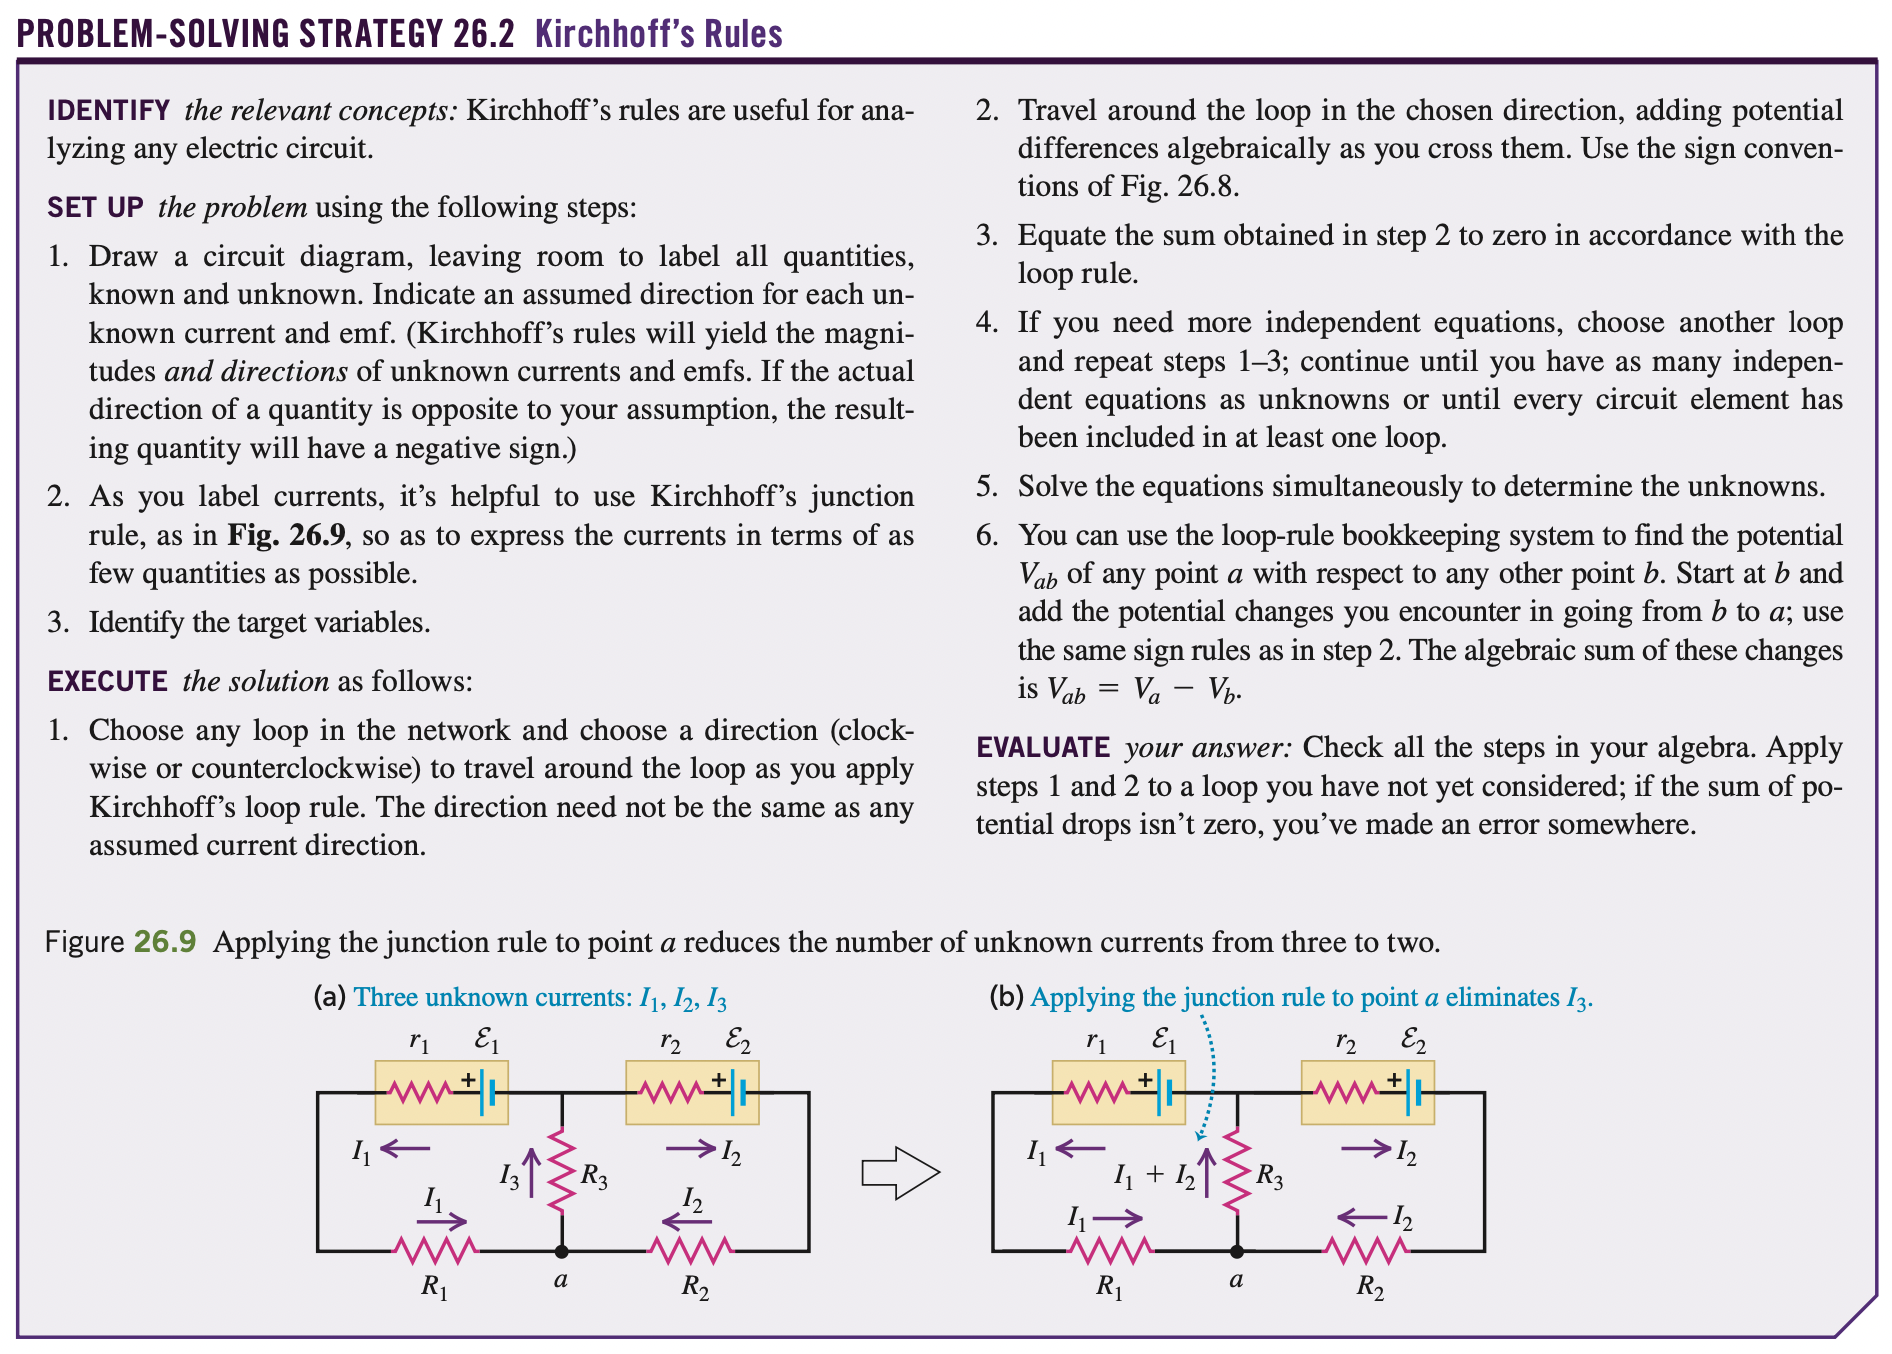
\includegraphics[scale=0.337]{kirchhoffs-rules}
\end{itemize}

\subsection{Electrical Measuring Instruments}

\begin{itemize}
  \item Many common devices measure current or potential difference with a \textbf{d'Arsonval galvanometer} which reports values via the deflection of a pointer

  \item The maximum deflection is called \textbf{full-scale deflection} and occurs at a particular current $I_\textrm{fs}$

  \item The device also has a resistance $R_c$

  \item A device that measures the current passing through it is called an \textbf{ammeter}

  \item An ideal ammeter would have 0 resistance so it doesn't affect the rest of the circuit, but real ammeters have a small, finite resistance

  \item An ammeter can be adjusted to measure currents larger than its full-scale reading by connecting a resistor in parallel so some current passes through the resistor — this is called a \textbf{shunt resistor} and obeys the relation \[I_\textrm{fs} R_\textrm{c} = (I_\textrm{a} - I_\textrm{fs}) R_\textrm{sh}\] where $I_\textrm{fs}$ is the device's full-scale current, $R_\textrm{c}$ is its coil resistance, $I_\textrm{a}$ is the desired full-scale current, and $R_\textrm{sh}$ is the resistance of the shunt resistor

  \item A device that measures the potential difference between two probes / terminals is called a \textbf{voltmeter}

  \item An ideal voltmeter would have infinite resistance so it doesn't affect the rest of the circuit, but real voltmeters have large, finite resistance

  \item A voltmeter can be adjusted to measure potential differences larger than its full-scale reading by connecting a resistor in series with it so the voltage drops before reaching the voltmeter — this obeys the relation \[V_\textrm{V} = I_\textrm{fs} (R_\textrm{c} + R_\textrm{s})\] where $V_\textrm{V}$ is the desired full-scale voltage, $I_\textrm{fs}$ is the device's full-scale current, $R_\textrm{c}$ is its coil resistance, and $R_\textrm{s}$ is the resistance of the resistor

  \item If you measure the current and voltage across an element simulateneously either the ammeter will be measuring the current across both the element and the voltmeter, or the voltmeter will be measuring the potential difference across both the element and the ammeter — either way you need to correct one of the measurements

  \item A device that measures resistance is called an \textbf{ohmmeter}

  \item A \textbf{potentiometer} is a device that can be used to measure an unknown emf via a known emf and a sliding contact attached to a resistor
\end{itemize}

\subsection{R-C Circuits}

\begin{itemize}
  \item A circuit that has a resistor and a capacitor in series is called an \textbf{R-C circuit}

  \item When charging the capacitor in an R-C circuit, the charge on the capacitor is given by \[q = C \mathcal{E} (1 - e^{-t / R C}) = Q_\textrm{f} (1 - e^{-t / R C})\] and the current in the circuit is given by \[i = \frac{\mathcal{E}}{R} e^{-t / R C} = I_0 e^{-t / R C}\]

  \item At $t = R C$ the capacitor has reached $1 - 1 / e$ of its final value and the current has decreased to $1 / e$ of its original value — this product $\tau = R C$ is a measure of how quickly the capacitor charges and is called the \textbf{time constant} or the \textbf{relaxation time}

  \item When discharging the capacitor in an R-C circuit, the charge on the capacitor is given by \[q = Q_0 e^{-t / R C}\] and the current in the circuit is given by \[i = -\frac{Q_0}{R C} e^{-t / R C} = I_0 e^{-t / R C}\]
\end{itemize}

\section{Magnetic Field and Magnetic Forces}

\begin{itemize}
  \item Electric forces act on electric charges whether they are moving or not but magnetic forces acts only on moving charges

  \item Electric forces arise in two stages: (1) a charge produces an electric field in the space around it, and (2) a second charge responds to this field

  \item Magnetic forces also arise in two stages: (1) a moving charge or a collection of moving charges (i.e. a current) produces a magnetic field, and (2) a second moving charge or current responds to this field
\end{itemize}

\subsection{Magnetism}

\begin{itemize}
  \item There is no experimental evidence that \textbf{magnetic monopoles} exist
\end{itemize}

\subsection{Magnetic Field}

\begin{itemize}
  \item Magnetic fields are vector fields represented by the symbol $\mathbf{B}$

  \item The direction of the field is the direction the North pole of a compass would point at that position

  \item For any magnet, $\mathbf{B}$ points out of its North pole towards its South pole

  \item The magnetic force on a moving charged particle is given by \[\mathbf{F} = q \mathbf{v} \times \mathbf{B}\]

  \item The unit of magnetic fields is the \textbf{tesla} where \[1\textrm{ tesla} = \qty{1}{T} = \qty{1}{N/A.m}\] or the \textbf{gauss} where \[\qty{1}{G} = \qty{1e-4}{T}\]

  \item When a charged particle moves through a region where both electric and magnetic fields are present the total force is the vector sum of the electric and magnetic forces \[\mathbf{F} = q (\mathbf{E} + \mathbf{v} \times \mathbf{E})\] this is called the \textbf{Lorentz force}
\end{itemize}

\subsection{Magnetic Field Lines and Magnetic Flux}

\begin{itemize}
  \item \textbf{Magnetic field lines} are to magnetic fields what electric field lines are to electric fields, however they don't show the force that would be exerted on a moving charge because that depends on the charge's velocity

  \item The magnetic flux through a surface is given by \[\Phi_B = \int \mathbf{B} \cdot d \mathbf{A}\]

  \item Magnetic flux uses the unit \textbf{weber} where \[\qty{1}{Wb} = \qty{1}{T.m^2} = \qty{1}{N.m/A}\]

  \item \textbf{Gauss's law for magnetism} states that the total magnetic flux through a closed surface is 0 \[\oint \mathbf{B} \cdot d \mathbf{A} = 0\]

  \item Sometimes we need to calculate the magnetic flux through an open surface in which case the direction of $d \mathbf{A}$ is ambiguous — in these scenarios we choose one direction to be positive and use that consistently
\end{itemize}

\subsection{Motion of Charge Particles in a Magnetic Field}

\begin{itemize}
  \item Magnetic forces do no work on point charges because they are always perpendicular to the charges' velocity

  \item The motion of a charge particle affected only by a magnetic force is always motion with constant speed

  \item The radius of a circular orbit in a magentic field is given by \[R = \frac{m v}{|q| B},\] the angular speed is given by \[\omega = \frac{|q| B}{m},\] and the frequency is given by \[f = \frac{\omega}{2 \pi} = \frac{|q| B}{2 \pi m}\]
\end{itemize}

\subsection{Applications of Motion of Charged Particles}

\begin{itemize}
  \item The speed for which there is no deflection in a velocity selector is \[v = \frac{E}{B}\]
\end{itemize}

\subsection{Magnetic Force on a Current-Carrying Conductor}

\begin{itemize}
  \item The magnetic force on a straight wire segment is given by \[\mathbf{F} = I \mathbf{l} \times \mathbf{B}\] where $\mathbf{l}$ is the vector length of the segment (points in the current direction)

  \item The magnetic force on a non-straight wire segment is given by \[\mathbf{F} = I \int d\mathbf{l} \times \mathbf{B}\]
\end{itemize}

\subsection{Force and Torque on a Current Loop}

\begin{itemize}
  \item The net force on a current loop in a uniform magnetic field is zero, however the net torque is not in general equal to zero

  \item The \textbf{magnetic dipole moment} or \textbf{magnetic moment} of a current loop is a vector perpendicular to the plane of the loop with direction determined by the current around the loop and right hand rule with magnitude \[\mu = I A\]

  \item A current loop or any any other object that experiences a magnetic torque in a magnetic field is called a \textbf{magnetic dipole}

  \item The magnetic torque experienced by a current loop is given by \[\boldsymbol{\tau} = \boldsymbol{\mu} \times \mathbf{B}\]

  \item The potential energy of a magnetic dipole in a magnetic field is \[U = -\boldsymbol{\mu} \cdot \mathbf{B}\]

  \item A coil consisting of $N$ planar loops close together is called a \textbf{solenoid} and its magnetic moment, potential energy, and torque are all multiplied by a factor of $N$
\end{itemize}

\setcounter{subsection}{8}
\subsection{The Hall Effect}

\begin{itemize}
  \item The Hall effect is described by the equation \[n q = \frac{-J_x B_y}{E_z}\] where $E_z$ is the induced electrostatic field in the conductor
\end{itemize}

\section{Sources of Magnetic Field}

\subsection{Magnetic Field of a Moving Charge}

\begin{itemize}
  \item The magnetic field due to a point charge with constant velocity is \[\mathbf{B} = \frac{\mu_0}{4 \pi} \frac{q \mathbf{v} \times \hat{\mathbf{r}}}{r^2}\] where $\mu_0$ is called the \textbf{magnetic constant}

  \item $\mu_0$ is approximately equal to $4 \pi \times 10^{-7}\, \unit{T . m / A}$
\end{itemize}

\subsection{Magnetic Field of a Current Element}

\begin{itemize}
  \item The \textbf{principle of superposition of magnetic fields} states that the total magnetic field caused by several moving charges is the vector sum of the fields caused by the individual charges

  \item The \textbf{Biot-Savart law} gives the magnetic field generated by a constant current \[\mathbf{B} = \frac{\mu_0}{4 \pi} \int \frac{I \,d\mathbf{l} \times \hat{\mathbf{r}}}{r^2}\]
\end{itemize}

\subsection{Magnetic Field of a Straight Current-Carrying Conductor}

\begin{itemize}
  \item The magnetic field near a long, straight, current-carrying conductor has direction as described by the right-hand rule and magnitude \[B = \frac{\mu_0 I}{2 \pi r}\]
\end{itemize}

\subsection{Force Between Parallel Conductors}

\begin{itemize}
\item The magnetic force per unit length between two long, straight, parallel, current-carrying conductors is \[\frac{F}{L} = \frac{\mu_0 I I'}{2 \pi r}\]

  \item Two parallel conductors carrying current in the same direction attract each other

  \item Two parallel conductors carrying current in opposite directions repel each other
\end{itemize}

\subsection{Magnetic Field of a Circular Current Loop}

\begin{itemize}
  \item The magnetic field on the axis of a current carrying loop is directed perpendicular to the plane of the loop as described by the right-hand rule and has magnitude \[B = \frac{\mu_0 I a^2}{2 \left( x^2 + a^2 \right)^{3/2}}\]

  \item The magnetic field of a coil consisting of $N$ loops has magnitude $N$ times that of a single loop

  \item Magnetic dipoles are also generators of magnetic fields with the magnetic field along the axis of $\boldsymbol{\mu}$ having the same direction as $\boldsymbol{\mu}$ and magnitude \[B = \frac{\mu_0 \mu}{2 \pi \left( x^2 + a^2 \right)^{3/2}}\]
\end{itemize}

\subsection{Ampere's Law}

\begin{itemize}
  \item \textbf{Ampere's law} relates the line integral of the magnetic field around a closed path to the net current enclosed by that path. If the currents are steady and no time-varying electric fields are present then \[\oint \mathbf{B} \cdot d\mathbf{l} = \mu_0 I_\textrm{encl}\]
\end{itemize}

\subsection{Applications of Ampere's Law}

\begin{itemize}
  \item The magnetic field of a long cylindrical conductor is \[B = \frac{\mu_0 I}{2 \pi} \frac{r}{R^2}\] inside the conductor and \[B = \frac{\mu_0 I}{2 \pi r}\] outside the conductor

  \item The magnetic field outside a solenoid is $0$ and inside is \[B = \mu_0 n I\] where $n$ is the number of windings per unit length

  \item The magnetic field outside a toroidal solenoid is $0$ and inside is \[B = \frac{\mu_0 N I}{2 \pi r}\] where $N$ is the number of turns of wire
\end{itemize}

\subsection{Magnetic Materials}

\begin{itemize}
  \item The \textbf{Bohr magneton} is a physical constant that represents the minimum magnetic moment and has the value \[\mu_B = \qty{9.274e-24}{A.m^2} = \qty{9.274e-24}{J/T}\]

  \item All magnetic moments must be an integer multiple of the Bohr megneton

  \item Some materials have atoms with net magnetic moments. In the presence of an external magnetic field these atoms experience a torque causing them to align with the field, generating a field of their own that increases the overall field strength. Such materials are called \textbf{paramagnetic materials}.

        \begin{itemize}
          \item The \textbf{magnetization} of a material is the density of magnetic moments \[\mathbf{M} = \frac{\boldsymbol{\mu}_\textrm{total}}{V}\] where $V$ is the volume of the material

          \item The additional magnetic field of a paramagnetic material is \[\mu_0 \mathbf{M} = \mu_0 \frac{\boldsymbol{\mu}_\textrm{total}}{V}\]

          \item If a current-carrying conductor is surrounded by paramagnetic material the total magnetic field is \[\mathbf{B} = \mathbf{B}_0 + \mu_0 \mathbf{M}\]

          \item The result of this additional magnetic field is that the total magnetic field is increased by a dimensionless factor $K_m$ called the \textbf{relative permeability} of the material

          \item Most equations can be adapted by multiplying by $K_m$

          \item To simplify this, the \textbf{permeability} $\mu = K_m \mu_0$ can be used instead

          \item The amount by which the relative permeability of a material differs from unity is called the \textbf{magnetic susceptibility} \[\chi_m = K_m - 1\]

          \item \textbf{Curie's law} describes how paramagnetic susceptibility is inversely proportional to temperature \[M = C \frac{B}{T}\] where $C$ is a material-specific constant and $T$ is the absolute temperature of the material
        \end{itemize}

  \item \textbf{Diamagnetic materials} oppose external magnetic fields, meaning they have a negative susceptibility and a relative permeability less than 1

        \begin{itemize}
          \item Diamagnetic materials are effectively temperature independent
        \end{itemize}

  \item \textbf{Ferromagnetic materials} contain ``domains'' in which atomic magnetic moments are aligned

        \begin{itemize}
          \item Applying an external magnetic field causes domains aligned with the field to grow and other domains to shrink

          \item As the magnitude of the external field is increased a point is reached where almost all atomic magnetic moments in the material are aligned with the field. Further increases to the magnitude of the field won't change the magnetization of the material — this is called saturation magnetization

          \item When a material is magnetized to saturation then the external field is reduced to zero, some magnetization remains — this behaviour is called \textbf{hysterisis} \\ 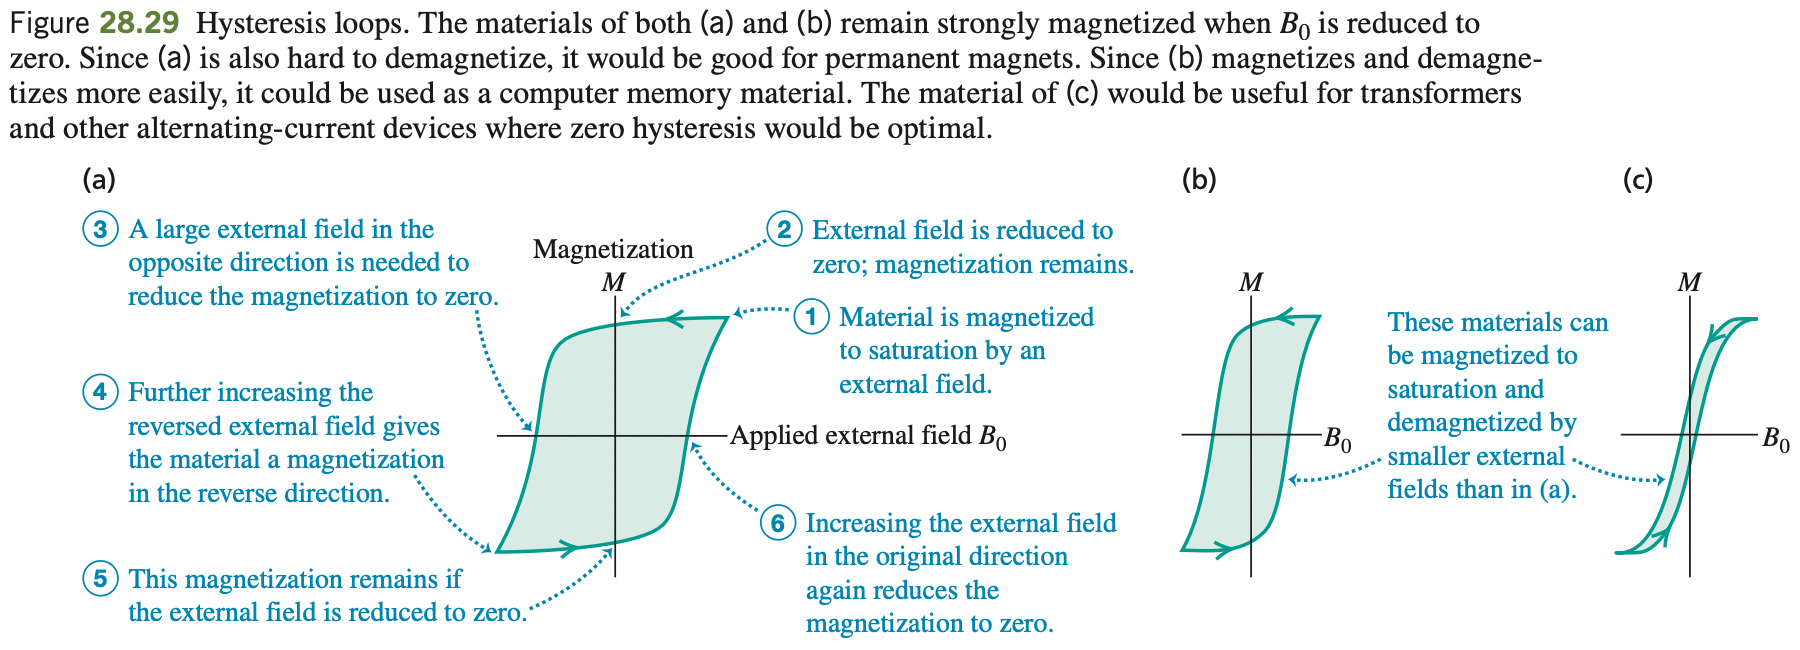
\includegraphics[scale=0.32]{hysterisis-loops}
        \end{itemize}
\end{itemize}

\section{Electromagnetic Induction}

\setcounter{subsection}{1}
\subsection{Faraday's Law}

\begin{itemize}
  \item \textbf{Faraday's law} states that the induced emf in a closed loop equals the negative of the time rate change of the magnetic flux through the loop \[\mathcal{E} = -\frac{d \Phi_B}{dt}\]

  \item The direction of induced emf is described by the right hand rule with the thumb in the direction of the area vector — a positive emf is in the direction of the fingers, a negative emf is in the opposite direction

  \item A coil of $N$ loops has $N$ times the magnetic flux and thus experiences $N$ times the induced emf
\end{itemize}

\subsection{Lenz's Law}

\begin{itemize}
  \item \textbf{Lenz's law} states that the direction of any magnetic induction effect is such as to oppose the cause of the effect

  \item If the change in flux is due to a changing magnetic field, the magnetic field resulting from the induced emf tries to ``undo'' the original change

  \item If the change in flux is due to changing area of the circuit, the current resulting from the induced emf experiences a magnetic force that tries to ``undo'' the original change
\end{itemize}

\subsection{Motional Emf}

\begin{itemize}
  \item Emf generated as a result of the conductor moving is called \textbf{motional emf} and has magnitude \[\mathcal{E} = v B L\] for a straight conductor of length $L$ and \[\mathcal{E} = \oint (\mathbf{v} \times \mathbf{B}) \cdot d\mathbf{l}\] for any conductor where $\mathbf{v}$ is the velocity of the infinitesimal conductor element and $\mathbf{B}$ is the magnetic field at its location
\end{itemize}

\subsection{Induced Electric Fields}

\begin{itemize}
  \item A changing magnetic field induces an electric field circumferential around the direction of the change

  \item Unlike electrostatic fields, \textbf{induced electric fields} or \textbf{nonelectrostatic fields} are non-conservative

  \item An alternative form of Faraday's law tells us the nature of the induced electric field \[\oint \mathbf{E} \cdot d \mathbf{l} = -\frac{d \Phi_B}{dt}\]

  \item Faraday's law describes two separate situations

        \begin{itemize}
          \item When a conductor moves through a static magnetic field, the magnetic force on the conductor's charge carriers induces an emf that opposes the movement

          \item When a magnetic field changes in a static conductor, an electric field is induced and hence an emf that opposes the change in flux
        \end{itemize}
\end{itemize}

\subsection{Eddy Currents}

\begin{itemize}
  \item Induced currents can circulate through the body of a conducting material as opposed to around a well-defined circuit. These are called \textbf{eddy currents}
\end{itemize}

\subsection{Displacement Current and Maxwell's Equations}

\begin{itemize}
  \item Ampere's law in the form \[\oint \mathbf{B} \cdot d \mathbf{l} = \mu_0 I_\text{encl}\] breaks in the case of a charging capacitor. If the integration surface is taken to intersect the wire at a higher potential then $I_\text{encl} = i_c$ (the conduction current) but if the integration path is kept the same and the integration surface changed to pass between the plates of the capacitor then $I_\text{encl} = 0$ \\ 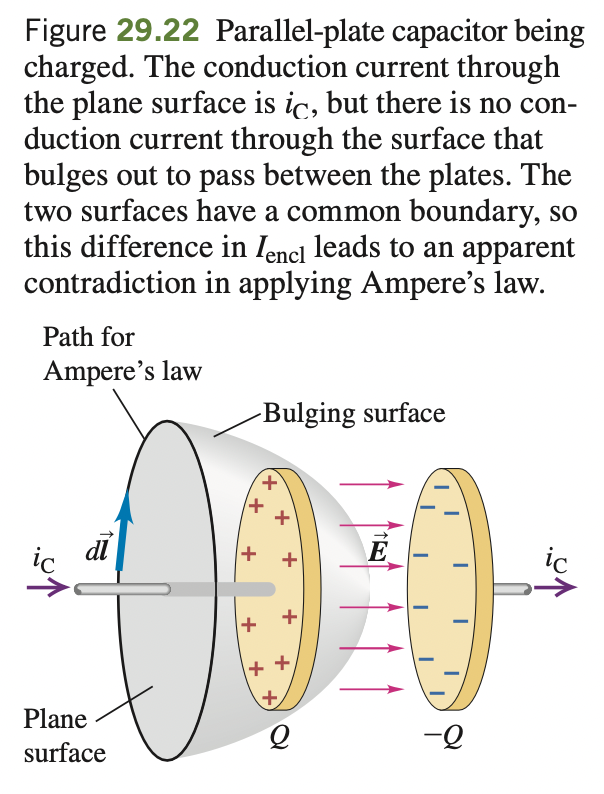
\includegraphics[scale=0.75]{amperes-law-capacitor}

  \item The generalized form of Ampere's law introduces a \textbf{displacement current} \[i_D = \epsilon_0 \frac{d \Phi_E}{dt}\] to account for the changing electric field between the plates of the capacitor \[\oint \mathbf{B} \cdot d \mathbf{l} = \mu_0 (i_C + i_D)_\text{encl}\] where $i_C$ is the conduction current and $i_D$ is the displacement current

  \item The displacement current actually exists and produces corresponding magnetic fields of its own

  \item \textbf{Maxwell's equations} describe all of the relationships between electric and magnetic fields

        \begin{itemize}
          \item Gauss's law for $\mathbf{E}$ \[\oint \mathbf{E} \cdot d \mathbf{A} = \frac{Q_\text{encl}}{\epsilon_0}\]

          \item Gauss's law for $\mathbf{B}$ \[\oint \mathbf{B} \cdot d \mathbf{A} = 0\]

          \item Faraday's law \[\oint \mathbf{E} \cdot d \mathbf{l} = -\frac{d \Phi_B}{dt}\]

          \item Generalized Ampere's law \[\oint \mathbf{B} \cdot d \mathbf{l} = \mu_0 (i_C + i_D)_\text{encl} = \mu_0 (i_C + \epsilon_0 \frac{d \Phi_E}{dt})_\text{encl}\]
        \end{itemize}
\end{itemize}

\section{Inductance}

\subsection{Mutual Inductance}

\begin{itemize}
  \item The \textbf{mutual inductance} of two coils is a proportionality constant that determines how much emf is generated in one coil from a changing current in the other coil \[\mathcal{E}_1 = -M \frac{di_2}{dt}\text{ and }\mathcal{E}_2 = -M \frac{di_1}{dt}\]

  \item Providing there isn't a magnetic material with a non-constant relative permeability present the mutual inductance only depends on the geometry of the two coils \[M = \frac{N_2 \Phi_{B2}}{i_1} = \frac{N_1 \Phi_{B1}}{i_2}\] where $N_n$ is the number of turns in coil $n$, $\Phi_{Bn}$ is the magnetic flux through a single loop of coil $n$, and $i_n$ is the current through coil $n$

  \item The SI unit of mutual inductance is the henry \[\qty{1}{H} = \qty{1}{Wb/A}\]
\end{itemize}

\subsection{Self-inductance and Inductors}

\begin{itemize}
  \item A current in a single isolated circuit establishes a magnetic field that causes a magnetic flux through the same circuit. This flux changes as the current changes, inducing an emf in the circuit. This \textbf{self-induced emf} opposes the change in current that caused it

  \item The \textbf{self-inductance} of a coil is \[L = \frac{N \Phi_B}{i}\] where $N$ is the number of loops in the coil, $\Phi_B$ is the average magnetic flux through each loop, and $i$ is the current

  \item The magnitude of self-induced emf can be calculated by rearranging the self-inductance

        \begin{align*}
          \frac{N \Phi_B}{i}      & = L                                         \\
          N \Phi_B                & = L i                                       \\
          N \frac{d \Phi_B}{dt}   & = L \frac{di}{dt}                           \\
          \Rightarrow \mathcal{E} & = -N \frac{d \Phi_B}{dt} = -L \frac{di}{dt}
        \end{align*}

  \item An \textbf{inductor} or \textbf{choke} is a device designed to have a particular self-inductance

  \item The potential difference between the terminals of an inductor is \[V = L \frac{di}{dt}\]

\item The self inductance of a solenoid is \[L = \frac{\mu_0 A N^2}{l}\]
\end{itemize}

\subsection{Magnetic-Field Energy}

\begin{itemize}
  \item The energy stored in an inductor is given be \[U = \frac{1}{2} L I^2\]

  \item The magnetic energy density in vacuum is \[u = \frac{B^2}{2 \mu_0}\] and in a material is \[u = \frac{B^2}{2 \mu}\]
\end{itemize}

\subsection{The R-L Circuit}

\begin{itemize}
  \item When an inductor is introduced into a circuit, the voltages, currents, and capacitor charges are in general functions of time rather than constants. However Kirchhoff's rules still apply at each moment in time

  \item An R-L circuit contains a resistor and an inductor in series

  \item After connecting a source of emf to an R-L circuit the current is \[i = \frac{\mathcal{E}}{R} (1 - e^{-(R / L) t})\] and its rate of change is \[\frac{di}{dt} = \frac{\mathcal{E}}{L} e^{-(R / L) t}\]

  \item After disconnecting a source of emf from an R-L circuit the current is \[i = I_0 e^{-(R / L) t}\] and its rate of change is \[\frac{di}{dt} = -\frac{I_0 R}{L} e^{-(R / L) t}\] where $I_0$ is its original current

  \item The \textbf{time constant} of an R-L circuit is the time it takes for the circuit to increase to 63\% of its final current after connecting a source of emf or decrease to 37\% of its original current after disconnecting a source of emf \[\tau = \frac{L}{R}\]
\end{itemize}

\subsection{The L-C Circuit}

\begin{itemize}
  \item An L-C circuit contains an inductor and a capacitor in series

  \item The circuit oscillates as in simple harmonic motion, with the capacitor's charge playing the role of elastic/gravitational potential energy and the current through the inductor playing the role of kinetic energy

\item The charge of the capacitor in an L-C circuit is given by \[q = Q \cos ( \omega t + \phi )\] and thus the current is given by \[i = -\omega Q \sin ( \omega t + \phi )\] where \[\omega = \sqrt{\frac{1}{L C}}\]
\end{itemize}

\subsection{The L-R-C Series Circuit}

\begin{itemize}
  \item An L-R-C series circuit is one where an inductor, resistor, and capacitor are in series

  \item The circuit oscillates as in damped harmonic motion

  \item The terms underdamped, critically damped, and overdamped apply the same as they do in mechanical damped harmonic oscillation

\item The angular frequency of an L-R-C circuit is \[\omega' = \sqrt{\frac{1}{L C} - \frac{R^2}{4 L^2}}\]
\end{itemize}

\section{Alternating Current}

\subsection{Phasors and Alternating Currents}

\begin{itemize}
  \item An \textbf{ac source} is any device that supplies a sinusoidally varying voltage \[v = V \cos \omega t\] or current \[i = I \cos \omega t\] where $v$ and $i$ are the instantaneous voltage and current and $V$ and $I$ are the voltage and current amplitude, respectively

  \item In a \textbf{phasor diagram} the value of a quantity that varies sinusoidally with time is represented by the projection onto a horizontal axis of a vector known as a \textbf{phasor} which has length equal to the amplitude of the quantity and constant angular speed $\omega$

  \item The \textbf{rectified average current} is defined such that after any whole number of cycles, the total charge that flows is the same as if the current was constant with a value equal to \[I_\text{rav} = \frac{2}{\pi} I \approx 0.637 I\]

  \item The \textbf{root-mean-square current} is obtained by squaring the current, taking the average value of the squared current, and taking the square root of that average. For ac currents \[I_\text{rms} = \frac{I}{\sqrt{2}}\] and \[V_\text{rms} = \frac{V}{\sqrt{2}}\]
\end{itemize}

\subsection{Resistance and Reactance}

\begin{itemize}
  \item \textbf{Reactance} is the opposition presented to alternating current by inductance or capacitance. It is similar to resistance in that it results in a smaller current for the same applied voltage, but it doesn't result in the dissipation of electrical energy as heat.

  \item The amplitude of voltage across a resistor in an ac circuit is \[V_R = I R\] and the instantaneous voltage is \[v_R = i R = (IR) \cos \omega t = V_R \cos \omega t\] so the voltage is in phase with the current

  \item The amplitude of voltage across an inductor in an ac circuit is \[V_L = I \omega L\] and the instantaneous voltage is

        \begin{align*}
          v_L & = L \frac{di}{dt}                                         \\
              & = L \frac{d}{dt} (I \cos \omega t)                        \\
              & = -I \omega L \sin \omega t                               \\
              & = I \omega L \cos \left( \omega t + \frac{\pi}{2} \right) \\
              & = V_L \cos \left( \omega t + \frac{\pi}{2} \right)
        \end{align*}

        so the voltage is out of phase with the current, leading it by $\ang{90}$.

  \item The \textbf{inductive reactance} of an inductor is defined as \[X_L = \omega L\] which lets the amplitude of voltage be written in the same form as that of a resistor \[V_L = I X_L\]

  \item The inductive reactance is a measure of the self-induced emf that opposes any change in current — greater angular frequency $\omega$ or inductance $L$ results in greater opposition

  \item The ampltiude of voltage across a capacitor in an ac circuit is \[V_C = \frac{I}{\omega C}\] and the instantaneous voltage is

        \begin{align*}
          v_C & = \frac{1}{\omega C} \sin \omega t                                \\
              & = \frac{1}{\omega C} \cos \left( \omega t - \frac{\pi}{2} \right) \\
              & = V_C \cos \left( \omega t - \frac{\pi}{2} \right)
        \end{align*}

        so the voltage is out of phase with the current, lagging it by $90^{\circ}$.

  \item The \textbf{capacitive reactance} of a capacitor is defined as \[X_C = \frac{1}{\omega C}\] which lets the amplitude of voltage be written in the same form as that of a resistor \[V_C = I X_C\]

  \item The capacitive reactance is measure of the voltage produced by the build up of charge on the plates of the capacitor which opposes current — greater angular frequency $\omega$ or capacitance $C$ results in less opposition
\end{itemize}

\subsection{The L-R-C Series Circuit}

\begin{itemize}
  \item An L-R-C series circuit is one that contains an inductor, a resistor, and a capacitor in series

  \item In the phasor diagram for such a circuit, the inductor phasor leads the current phasor by $\ang{90}$, the resistor phasor is parallel with it, and the capacitor phasor lags by $\ang{90}$

  \item The instantaneous voltage of any ac circuit is equal to the projection of the vector sum of the components' phasors

  \item The \textbf{impedance} $Z$ of an ac circuit is a measure of its opposition to ac current due to the combined effect of resistance and reactance. It is defined as the ratio of the voltage amplitude to the current amplitude in the circuit \[Z = \frac{V}{I} \Rightarrow V = I Z\]

  \item The impedance of an L-R-C series circuit is \[Z = \sqrt{R^2 + (X_L - X_C)^2} = \sqrt{R^2 + [\omega L - (1 / \omega C)]^2}\]

  \item The phase angle of voltage with respect to current in an L-R-C series circuit is \[\tan \phi = \frac{X_L - X_C}{R} = \frac{\omega L - 1 / \omega C}{R}\]

  \item The equations above are valid if a component is missing from an L-R-C series circuit

        \begin{itemize}
          \item If the resistor is missing, set $R = 0$

          \item If the inductor is missing, set $L = 0$

          \item If the capacitor is mising, set $C = \infty$
        \end{itemize}

  \item The above equations deal with ampitudes, but they can be modified to deal with rms values by dividing current and voltage by $\sqrt{2}$

  \item Kirchhoff's rules hold at each instance in an ac circuit
\end{itemize}

\subsection{Power in Alternating-Current Circuits}

\begin{itemize}
  \item The instantaneous power delivered to an ac circuit element is \[p = vi\]

\item The average power delivered to an ac circuit consisting only of a resistor is \[P_\text{av} = \frac{1}{2} V I = \frac{V}{\sqrt{2}} \frac{I}{\sqrt{2}} = V_\text{rms} I_\text{rms}\]

  \item Because $V_\text{rms} = I_\text{rms} R$, the above can also be expressed as \[P_\text{av} = I_\text{rms}^2 R = \frac{V_\text{rms}^2}{R} = V_\text{rms} I_\text{rms}\]

  \item Because the voltage across an inductor leads the current by $\ang{90}$, half the time the product $v i$ is positive and half the time it's negative and thus the average power delivered to an inductor is $0$

  \item When the voltage across an inductor is positive the magnetic field is being established and when it's negative the magnetic field is collapsing, returning energy back to the circuit

  \item Because the voltage across a capacitor lags the current by $\ang{90}$, half the time the product $v i$ is positive and half the time it's negative and thus the average power delivered to a capacitor is $0$

  \item When the voltage across a capacitor is positive charge is building up on the plates and when it's negative the charge is returning to the circuit

  \item The instantaneous power delivered to a circuit is

        \begin{align*}
          p & = v i                                                                       \\
            & = [V \cos (\omega t + \phi)] [I \cos \omega t]                              \\
            & = [V (\cos \omega t \cos \phi - \sin \omega t \sin \phi)] [I \cos \omega t] \\
            & = V I \cos \phi \cos^2 \omega t - V I \sin \phi \cos \omega t \sin \omega t
        \end{align*}

  \item The average value of $\cos^2 \omega t$ over one cycle is $\frac{1}{2}$ and $\cos \omega t \sin \omega t$ is equal to $\frac{1}{2} \sin 2 \omega t$, the average value of which over one cycle is $0$ so \[P_\text{av} = \frac{1}{2} V I \cos \phi = V_\text{rms} I_\text{rms} \cos \phi\]

  \item In other words, the average power delivered to a circuit is equal to $\frac{1}{2} I$ times $V \cos \phi$ which is the projection of the voltage phasor onto the current phasor, i.e. only the component of the voltage that is in phase with the current contributes to power

  \item The factor $\cos \phi$ is called the \textbf{power factor} of the circuit

  \item The power factor of an L-R-C circuit is equal to $R / Z$
\end{itemize}

\subsection{Resonance in Alternating-Current Circuits}

\begin{itemize}
  \item As the angular frequency $\omega$ of an ac source increases, $X_C$ decreases and $X_L$ increases. For one value they're equal meaning $Z = \sqrt{R^2 + (X_L - X_C)^2}$ is minimised and $I = V / Z$ is maximised. This behaviour is called \textbf{resonance} and the angular frequency at which $Z$ is minimised and $I$ is maximised is called the \textbf{resonance angular frequency} \[\omega_0 = \frac{1}{\sqrt{L C}}\]

  \item At the resonance angular frequency $V_C = I X_C$ and $V_L = I X_L$ are equal and opposite, meaning $V = V_R$ and all power in the circuit is delivered to the resistor
\end{itemize}

\subsection{Transformers}

\begin{itemize}
  \item A \textbf{transformer} uses magnetic induction to change a source voltage. \\ 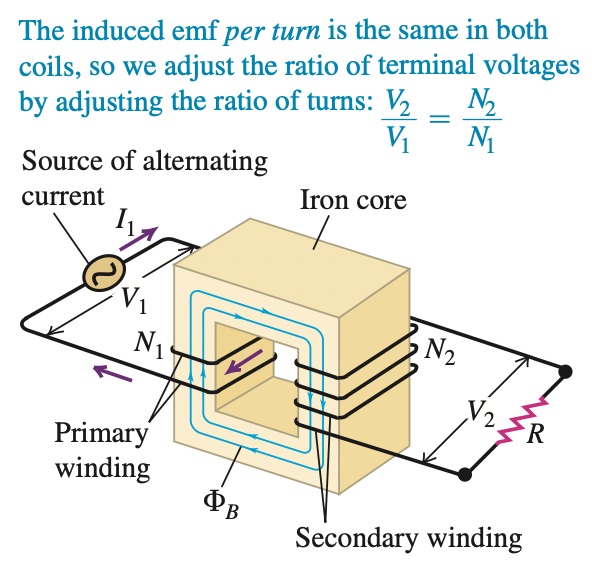
\includegraphics[scale=0.75]{transformer}

  \item The ratio of terminal voltages in a transformer is given by \[\frac{V_2}{V_1} = \frac{N_2}{N_1}\]

  \item If $N_2 > N_1$ then $V_2 > V_1$ and it's called a step-up transformer. If $N_2 < N_1$ then $V_2 < V_1$ and it's called a step down transformer.

  \item The power delivered to both windings is equal \[V_1 I_1 = V_2 I_2\]
\end{itemize}

\end{document}